\documentclass[11pt]{article}
\usepackage{amsmath, amssymb, graphicx, float, geometry}
\usepackage{booktabs}
\usepackage{hyperref}
\usepackage{graphicx}
\geometry{margin=1in}

\title{Multi-Particle Social Force Simulation via Cost Function Minimization}
\author{Jacob Carton}
\date{}

\begin{document}

\maketitle

\section{Introduction}

In this project, we extend single-particle cost-function motion to a multi-particle system.
The formulation is inspired by the Social Force Model introduced by Helbing and Moln\'ar,
but reinterpreted entirely through cost-function minimization.

Rather than integrating physical forces directly, particle motion emerges from gradient
descent on a composite cost function consisting of:

\begin{itemize}
\item Goal attraction
\item Wall penalty terms
\item Social interaction penalties
\end{itemize}

The objective is to compare isotropic and anisotropic social force models and analyze
emergent collective behavior.

\section{Mathematical Formulation}

Let $x_i \in \mathbb{R}^2$ denote the position of particle $i$.

\subsection{Total Cost Function}

\[
C_i(x_i) =
C_{\text{goal}}(x_i)
+
C_{\text{walls}}(x_i)
+
\sum_{j \ne i} C_{\text{social}}(x_i, x_j)
\]

Particles update via gradient descent:

\[
x_i^{k+1} =
x_i^{k} - \alpha \nabla_{x_i} C_i
\]

\section{Goal Term}

We use a quadratic attraction:

\[
C_{\text{goal}}(x_i)
=
\frac{k_g}{2} \|x_i - x_i^{goal}\|^2
\]

Gradient:

\[
\nabla C_{\text{goal}} = k_g (x_i - x_i^{goal})
\]

\section{Wall Penalty}

Let $d(x)$ denote distance to nearest wall.

We use an exponential barrier:

\[
C_{\text{wall}}(x)
=
A_w e^{-d(x)/B_w}
\]

Gradient:

\[
\nabla C_{\text{wall}} =
- \frac{A_w}{B_w}
e^{-d/B_w} \nabla d
\]

\section{Isotropic Social Forces}

\subsection{Quadratic Repulsion}

\[
C_{ij}
=
\begin{cases}
\frac{1}{2}(R - d_{ij})^2 & d_{ij} \le R \\
0 & d_{ij} > R
\end{cases}
\]

\subsection{Exponential Repulsion}

\[
C_{ij} = A \exp\left(-\frac{d_{ij}}{B}\right)
\]

\section{Anisotropic Social Forces}

Let $v_i$ be velocity and $\hat v_i = \frac{v_i}{\|v_i\|}$.

\[
C_{ij}
=
\left(
1 + \beta \max\left(0,
\hat v_i \cdot
\frac{x_j - x_i}{\|x_j - x_i\|}
\right)
\right)
\phi(d_{ij})
\]

This introduces directional bias and breaks symmetry.

\section{Experiments}

\subsection{Open Space}

We simulate $N=12$ particles moving toward a common goal.

\begin{figure}[h!]
	\centering
	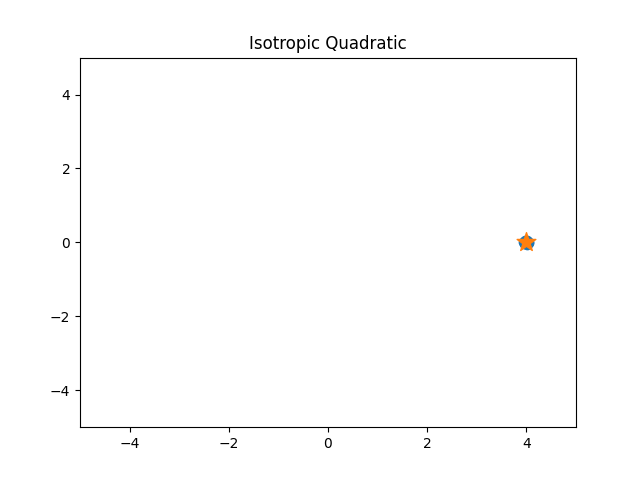
\includegraphics[width=0.8\textwidth]{iso-quad.png}
	\caption{This shows the quadric repulsion of an isotropic force}
	\label{fig:iso-quadratic}
\end{figure}

\begin{figure}[h!]
	\centering
	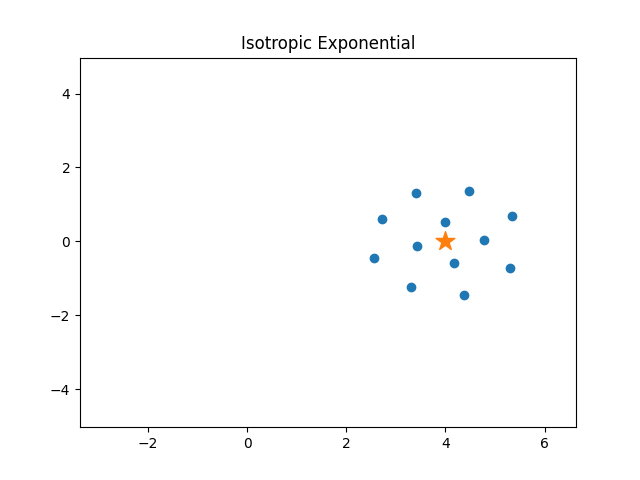
\includegraphics[width=0.8\textwidth]{iso-expo.png}
	\caption{This shows the exponential repulsion of an isotropic force}
	\label{fig:iso-exponential}
\end{figure}

\begin{figure}[h!]
	\centering
	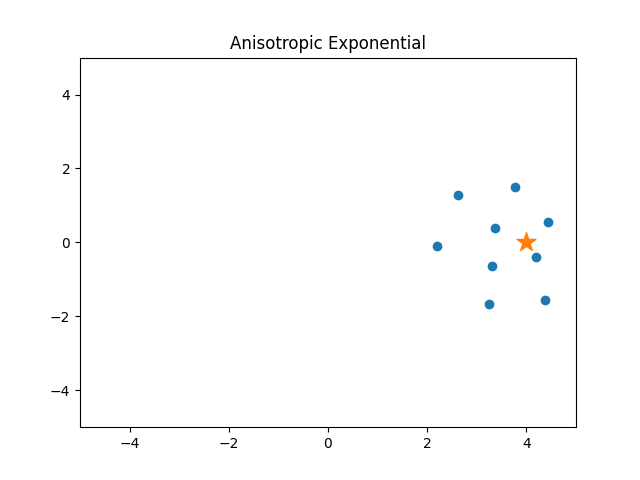
\includegraphics[width=0.8\textwidth]{aniso-expo.png}
	\caption{This shows the anisotropic exponential repulsion}
	\label{fig:anisotropic-exponential}
\end{figure}

\subsection{Corridor Bottleneck}

Walls create a narrow passage.
We compare isotropic and anisotropic models.

\section{Results and Analysis}

\subsection{Symmetry}

Isotropic fields are radially symmetric.
Anisotropic fields break symmetry.

\subsection{Oscillations}

Isotropic models show head-on oscillations.
Anisotropic reduces deadlocks by prioritizing forward motion.

\subsection{Corridor Behavior}

Isotropic: clogging and symmetry-induced stalls.
Anisotropic: smoother lane formation.

\subsection{Trade-offs}

Advantages:
\begin{itemize}
\item More realistic behavior
\item Reduced oscillations
\end{itemize}

Disadvantages:
\begin{itemize}
\item Velocity dependence introduces sensitivity
\item Not strictly conservative
\end{itemize}

\section{Conclusion}

Multi-particle motion emerges from cost-function design alone.
Anisotropic social forces improve stability and realism but introduce additional complexity.
Potential-field methods remain limited by local minima and symmetry-induced deadlocks.

\end{document}